As our system enables to handle transparent visualization of molecular surface in real-time, it provides the users with the possibility to explore the MD simulation instantly, without any precomputation or making previews on selected time steps.
The latter technique is often used for creating an overview of an observed process (e.g., time changes of a protein tunnel, following the ligand path, observing the trajectories of water molecules, etc.).
The user selects a subset of the original MD simulation consisting of each $n-$th time step and the given task is performed only on this subset.
Depending on the selected $n$ value, it can give the user a decent overview information. 
But there is always a risk that the substantial parts of the simulation were omitted.

The real-time exploration of the transparent molecular surface and inner cavities has the following advantages:
\begin{itemize} 
\item The MD simulation can be observed in real time which enables the user to interactively adjust the appearance and viewpoint.
\item The highly transparent molecular surface removes the necessity of using clip planes which are often used for exploration of the inner molecular environment.
\item The user has the full control of the animation process. 
\end{itemize}

%In consequence, our system enables to reach similar results in real-time. 
%In one aspect it even overcomes the existing solution as the users can interactively manipulate with the scene on the fly~--~perform scene transformations, change the appearance of the protein and ligand, or change the probe size used for the generation of protein surface.

%Figure \ref{fig:animation} (bottom) shows one time step of the animation generated using the same dataset (\textit{LINB acetone} simulation consisting of 9256 time steps) as for the top part of this Figure.

%\begin{figure}[htb]
%  \centering
%  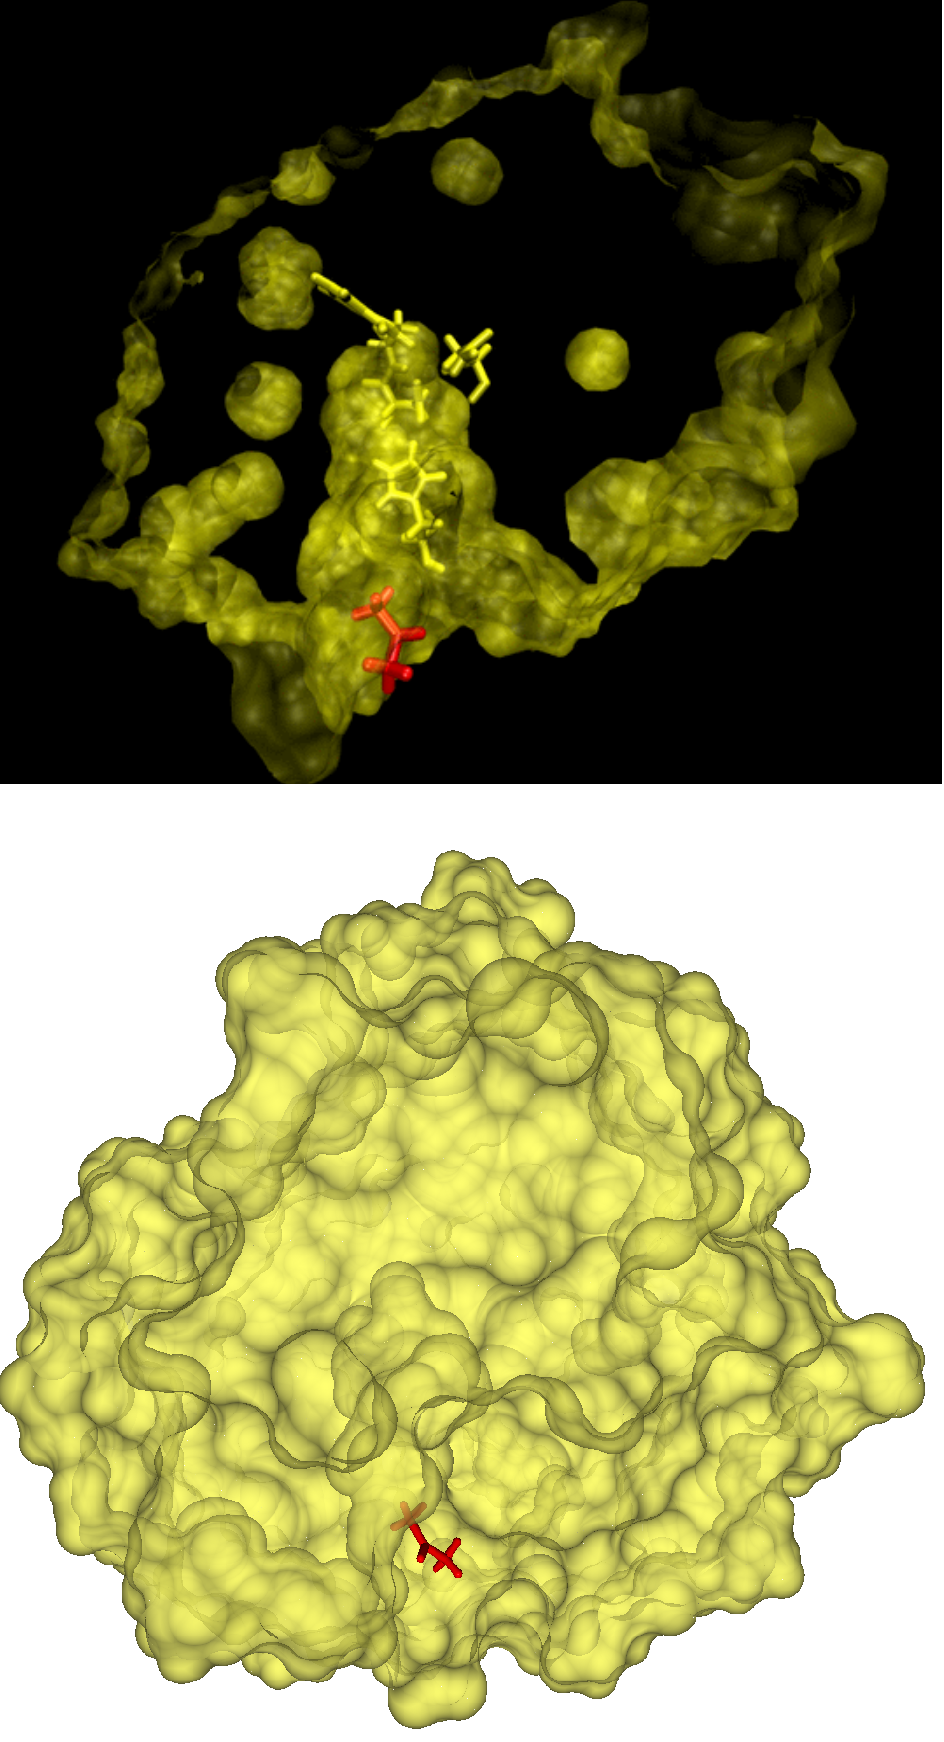
\includegraphics[width=2.5in]{image/animation.png}
%  \caption{Top: One time step from the animation aiming to show the penetration of the ligand to the protein active site. For better insight, different representations of the molecule and the ligand, surface transparency, clip plane, and different coloring was used. Bottom: One time step of the animation generated using our algorithm. It shows the same molecule and its dynamics. By enabling the interactive manipulation with the scene within the animation, the user can clearly see the transportation route without the necessity to use any clip plane.}
%	\label{fig:animation}
%\end{figure}

\subsection{Performance Analysis}
\label{sec:performance}

We tested our technique on commodity hardware to show that it enables the users to solve their tasks in real-time without high hardware requirements.
The tests were performed using Intel Core i5 760 (2.80 GHz) with 4 GB of RAM and NVIDIA GeForce 680 GTX with 4 GB of VRAM as a graphics card.
For rendering, we used the resolution of 1024 $\times$ 768 and we fitted the molecule to cover most of the rendered image.
%Regarding transparency, we limited the maximum depth complexity to 24 fragments per pixel.
The results of our measurements for both static and dynamic\textcolor{red}{s} molecules are presented in Table~\ref{tab:static}.
We choose the static structures from the Protein Data Bank (PDB)~\cite{sussman1998protein} so the performance of our technique could be easily compared with other existing or new approaches on the same dataset.

\textcolor{green}{
In Table~\ref{tab:speedup}, we compare overall performance of our technique to the method presented by Kauker et al.~\cite{kauker2013rendering} as it is the only existing method that enables correct transparency of the SES in real-time.
When compared to state-of-the-art methods~\cite{lindow2010accelerated}~\cite{krone2011parallel} for SES visualization, our method performs in the surface computation part similarly to the algorithm we came from~\cite{krone2011parallel} (see Tab.~\ref{tab:static}).
The performance of the ray-casting is not directly comparable to the methods.
We test twice as many intersections to obtain both front and back fragments and our intersection tests (especially for spherical patches) need to be more complex than those used by techniques that do not render the surface using full transparency.
}

\setlength{\tabcolsep}{4.5pt}

\begin{table}[htb]
  \caption{Performance of our technique for static and dynamic (*) structures.
	The table shows timings of the key phases of our method: surface computation (CB), cavity computation (SG), area estimation and ray-casting (RC).
	For ray-casting, we also include fill rate (FR).
	Performance of our technique does not vary significantly for static or dynamic data as it operates on a per-frame basis.}
  \label{tab:static}
  \scriptsize
  \begin{center}
    \begin{tabular}{cccccccc}
      Molecule & \# Atoms & FR & CB & SG & Area & RC & Total \\
			%        &       & buildup  & graph   & Area & casting &       \\
							&      & (\%) & (ms)     & (ms)    & (ms) & (ms) & (FPS) \\
    \hline
      1OGZ      &  {\tweakedsim}1000 & 41.5 &  3.5 & 0.3 & 0.2 &  5.9 & 47.8 \\
      1VIS      &  {\tweakedsim}2500 & 50.5 &  5.9 & 0.8 & 0.2 &  9.5 & 34.1 \\
			LINB-ACE* &  {\tweakedsim}4500 & 29.8 & 17.2 & 0.6 & 0.2 &  9.3 & 22.6 \\
      4ADJ      & {\tweakedsim}10000 & 43.1 & 21.0 & 4.1 & 0.4 & 20.2 & 15.2
    \end{tabular}
  \end{center}
\end{table}

\begin{table}[htb]
  \caption{Speedup of our technique in comparison to Kauker et al.~\cite{kauker2013rendering}.
	The table shows number of depth layers (DL), rendering speeds (FPS) of both methods and the relative speedup. Fill rate (FR) which significantly affects performance of ray-casting is also included.}
  \label{tab:speedup}
  \scriptsize
  \begin{center}
    \begin{tabular}{cc|ccc|ccc|c}
		           &          & \multicolumn{3}{c|}{Our} & \multicolumn{3}{c|}{Kauker et al.} & \\
      Molecule & \# Atoms & FR & DL & FPS & FR & DL & FPS & Speedup \\
			%        &       & buildup  & graph   & Area & casting &      \\
							 &          & (\%) &  &     & (\%) &  &     &         \\
    \hline
      1YV8 &   {\tweakedsim}650 & 38.6 & 12 & 40.1 & 18.0 & 117 & 31.0 & 1.29 \\
      1VIS &  {\tweakedsim}2500 & 52.7 & 15 & 34.1 & 48.7 & 135 & 11.2 & 3.04 \\
      4ADJ & {\tweakedsim}10000 & 41.5 & 19 & 20.2 & 42.8 & 188 &  6.2 & 3.26
    \end{tabular}
  \end{center}
\end{table}

Our technique was implemented mainly using OpenGL employing GLSL compute shaders as GPU kernels.
We also utilized \textcolor{red}{(used)} OpenCL to implement a kernel which computes the positions of spherical triangles in the original algorithm \cite{krone2011parallel}.
The GLSL implementation of this kernel performed for a molecule with {\tweakedsim}10000 atoms about 5x slower than the OpenCL/CUDA one.
Based on the performed tests we assume that the key reason for such performance loss is the extensive use of the global memory in the kernel which is handled differently in OpenGL and OpenCL/CUDA.

\subsubsection{Discussion of Limitations}
From the results, it can be seen that in terms of performance, the main limitation of our technique is the ray-casting of the computed surface.
More specifically, the most demanding part is the rendering of spherical and toroidal patches that takes together 75-80\% of the whole rendering time.
We anticipate that the performance of ray-casting these patches could be improved by using tighter bounding boxes for them when splatting.
In fact, we employ bounding squares for both spheres containing spherical patches and visibility spheres containing visible parts of tori.
In this way, the computation of ray-primitive intersection is evaluated multiple times for spheres and tori that form more than one surface patch.

\subsubsection{Improved Memory Complexity}

As a side effect of exploiting the hash data structure (Sec.~\ref{sec:ecb}) for storing spherical triangles, our technique consumes less GPU memory than the original approach we used as a basis.
This is due to the fact that the original method uses a linear buffer to store the spherical triangles.
An index into this buffer, i.e., position where a triangle is stored, is computed based on the $i$ and $j$ indices of spheres $i < j < k$ that formed the triangle.
The range of $j$ is optimized in terms of limiting the maximal number of neighbors ($maxNeighbors$) that a sphere can have, so that the range of $j$ can be remapped to $\left[0, maxNeighbors\right)$.
There is also a limit on the total number of triangles ($maxTriangles$) that can be stored for each pair of spheres.
Putting it all together, the memory complexity of the original data structure is:

\begin{equation}
|A| \cdot maxNeighbors \cdot maxTriangles,
\end{equation}

where $|A|$ is the number of atoms of the molecule and the typical settings for the other two constants are $maxNeighbors = 64$, $maxTriangles = 64$.
We adopted this settings from the MegaMol visualization framework~\cite{grottel2015megamol}.

On the other hand, we store the computed triangles linearly in an array and for each triangle, we additionally store three hash records. 
The memory complexity of our hash structure is therefore:

\begin{equation}
|T| + hashFreeRatio \cdot 3 |T|,
\end{equation}

where $|T|$ is the number of computed spherical triangles and the typical setting for the constant is $hashFreeRatio = 2$. 

To be able to compare the complexity of these two data structures, we estimate the ratio between the number of atoms and the number of triangles to be (taken from experiments):

\begin{equation}
\frac{|A|}{|T|} > \frac{1}{4}.
\end{equation}

Then, the complexity ratio can be expressed as:

\begin{equation}
\frac{|A| \cdot maxNeighbors \cdot maxTriangles}{|T|(1 + 3 \cdot hashFreeRatio)} > \frac{64^2}{28} > 146,
\end{equation}

which yields that the original structure is more than 100 times larger for only 64 neighbors.
Actually, our maximum neighbor count is 128 to be able to compute the surface of molecules that contains hydrogens, which is a typical case for data produced by molecular dynamics simulations.


\subsection{Discussion}
When the results of the algorithm were evaluated by the domain experts, they confirmed that our solution is highly practical with respect to the exploration of molecular surface and inner cavities because the time to complete this task is reduced dramatically.
The agreed that this approach has a big potential in the field of studying protein-protein interactions where the reactions happen on the protein surfaces.
Therefore, studying of the shape of these surfaces and their changes over time is substantial in this case.
Moreover, they also appreciated the visual appearance which they considered to be more appealing than the previous solutions.
They confirmed that our approach can be directly used for creating presentation materials, such as images to publications or animations for presentations.

The domain experts were also asked to identify the weak points of our current solution.
They agreed that when using a highly transparent molecular surface, it can be hard to assess the position of penetrating structures (ligands) when using only one viewpoint.
In other words, the user has to manipulate with the structure in order to decide if the ligand is still located in the outer solvent or if it already penetrated to the inner part of the protein.
However, this situation is caused due to the transparency itself and a solution has to be based on a combination with other methods.
This opens one of the possible directions for the future extension.
Another possible extension suggested by the biochemists is to enable a selection of an interesting cavity (e.g., containing the active site) and focus on its changes.
According to the domain experts, our algorithm could be also extended to be applicable to other voids in proteins, namely tunnels.


%\subsection{Case Study~--~Real-time visual exploration of MD simulation}
%The case study deals with the situation when the biochemists want to visually explore the inner processes occurring inside the molecule. 
%An example of such a process can be the penetration of a small molecule (ligand) into the active site of the protein where the ligand reacts with the protein and the product of such reaction can form the basis of new chemical matters, e.g., new drugs. 
%The current workflow generating the desired visual appearance of the animation showing such processes consists of many trial and error attempts, which makes the whole workflow very lengthy. 
%To describe this process in more detail, the biochemists start in the first time step of the whole simulation and try to manually determine the best viewpoint.
%As the view inside the molecule, where the processes usually occur, is crucial, they utilize clip planes to achieve this.
%The manual setting of the clip planes introduces other possible error to the final animation.
%The dynamic movements of the molecule can cause its rotation and the clip plane settings in the first time step might have completely wrong positions in the following steps.
%When all the visual parameters are set in the first frame (Fig.~\ref{fig:animation}), the biochemists use an offline rendering tool for generating the whole animation.
%In this phase they do not posses any control of this process so it is impossible to detect an error inside the animation and stop the generation.
%These errors, such as occlusions or wrong clip plane positions, are detected when playing the final animation.
%The only solution is to adjust the input settings and launch the whole process once again.
%For better illustration, in case of the example video (from which Figure~\ref{fig:animation} (top) is captured), it took two days to produce the solution which comprehensibly shows the whole process of ligand penetration to the protein active site.

